\documentclass[conference]{IEEEtran}

% Packages
\usepackage[utf8]{inputenc}
\usepackage[english]{babel}
\usepackage{amsmath}
\usepackage{amsfonts}
\usepackage{amssymb}
\usepackage{amsthm}
\usepackage{pdfpages}
\usepackage{graphicx}
\usepackage{epstopdf}
\usepackage{listings}
\usepackage{cite}
\usepackage{enumerate}
\usepackage{scientific}
\usepackage[colorlinks=false]{hyperref}
\usepackage{bookmark}

\usepackage[]{mcode}	%Matlab Code
\usepackage{tikz,pgfplots}	%Tikz
\usepackage{paralist}	% Auzählungen

% Bookmark Setup
\bookmarksetup{numbered}

% PDF Setup
\hypersetup{pdftitle={Assignment 2}, pdfsubject={Documentation of 2nd Homework}, pdfauthor={Stefan Röhrl}, pdfkeywords={MLIR Assignment 2}, pdfcreator={LaTeX}, hidelinks}


\begin{document}
%
% cite all references
%\nocite{*}
%
% paper title
% can use linebreaks \\ within to get better formatting as desired
\title{MACHINE LEARNING IN ROBOTICS\\ Assignment 2}

\author{\IEEEauthorblockN{Stefan Röhrl}
\IEEEauthorblockA{Technische Universität München, Arcisstraße 21, Munich, Germany\\
Email: stefan.roehrl@tum.de}}

% use for special paper notices
%\IEEEspecialpapernotice{(Invited Paper)}

% make the title area
\maketitle

\IEEEpeerreviewmaketitle

\section{Exercise}

\begin{flushleft}
Learned parameters for GMM after Expectation-Maximization.\\

Covariance Matrices:
$$
\Sigma_1 =
 \begin{pmatrix}
    3.946e-04 & 2.169e-04\\
	2.169e-04 & 1.277e-04
 \end{pmatrix}
$$

$$
\Sigma_2 =
 \begin{pmatrix}
    7.436e-04 & -5.914e-04\\
	-5.914e-04 & 6.098e-04
 \end{pmatrix}
$$

$$
\Sigma_3 =
 \begin{pmatrix}
	1.083e-03 & -4.244e-04\\
	-4.244e-04 & 2.431e-04
 \end{pmatrix}
$$

$$
\Sigma_4 =
 \begin{pmatrix}
	1.748e-04 & 2.616e-04\\
	2.616e-04 & 3.976e-04
 \end{pmatrix}
$$
\\
Means:
$$
\mu_1 =
 \begin{pmatrix}
	-1.470e-02 \\ -7.963e-02
 \end{pmatrix}
$$

$$
\mu_2 =
 \begin{pmatrix}
	-1.937e-02 \\ -1.664e-02
 \end{pmatrix}
$$

$$
\mu_3 =
 \begin{pmatrix}
	2.619e-02 \\ 6.173e-02
 \end{pmatrix}
$$

$$
\mu_4 =
 \begin{pmatrix}
	-4.319e-02 \\ 4.459e-02
 \end{pmatrix}
$$
Priors:
$$ \pi_1 = \begin{pmatrix} 2.012e-01 \end{pmatrix} $$

$$ \pi_1 = \begin{pmatrix} 2.971e-01 \end{pmatrix} $$

$$ \pi_1 = \begin{pmatrix} 2.617e-01 \end{pmatrix} $$

$$ \pi_1 = \begin{pmatrix} 2.400e-01 \end{pmatrix} $$
\end{flushleft}

\begin{figure}[h!]
  	\centering
    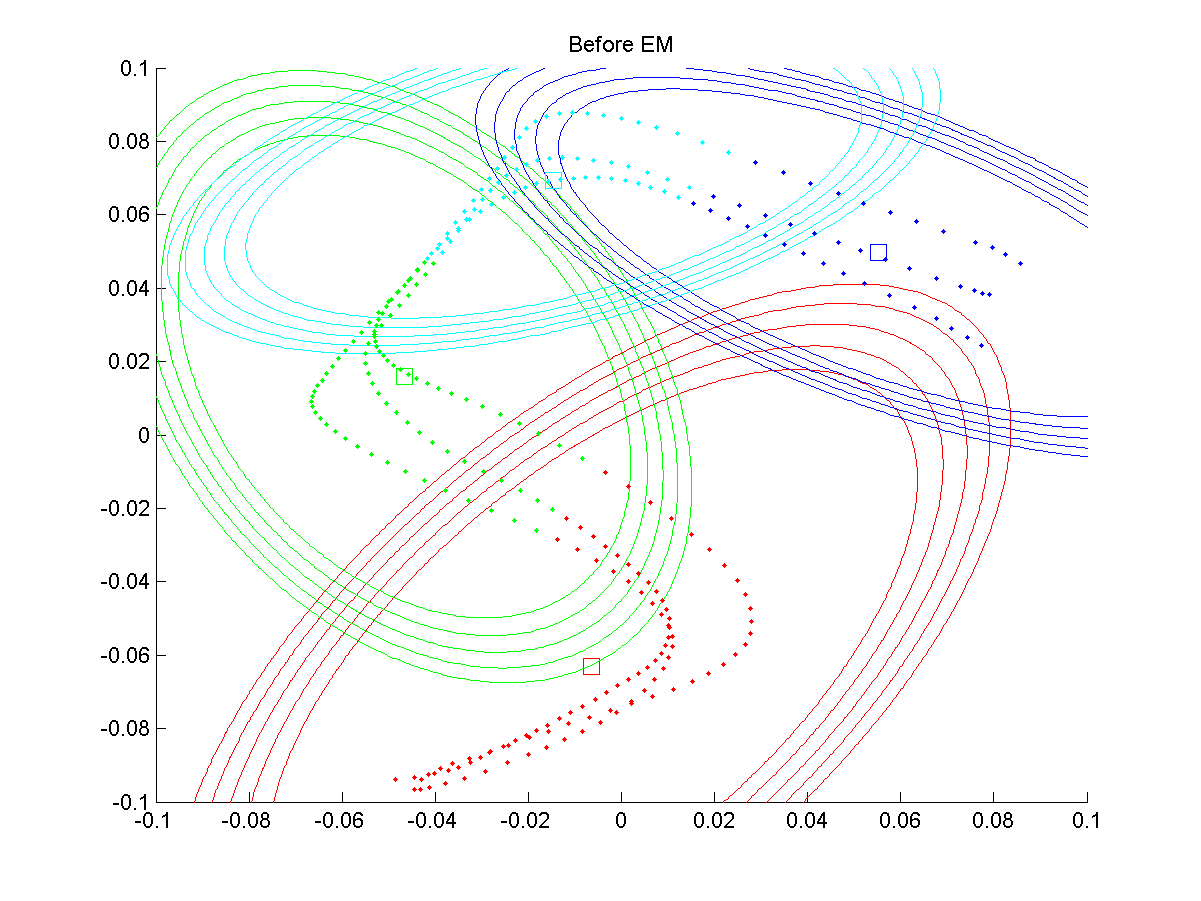
\includegraphics[width=0.5\textwidth]{img/1before_em.png}
    \caption{Gaussians and clusters before EM}
    \label{fig:before_em}
\end{figure}

\begin{figure}[h!]
  	\centering
    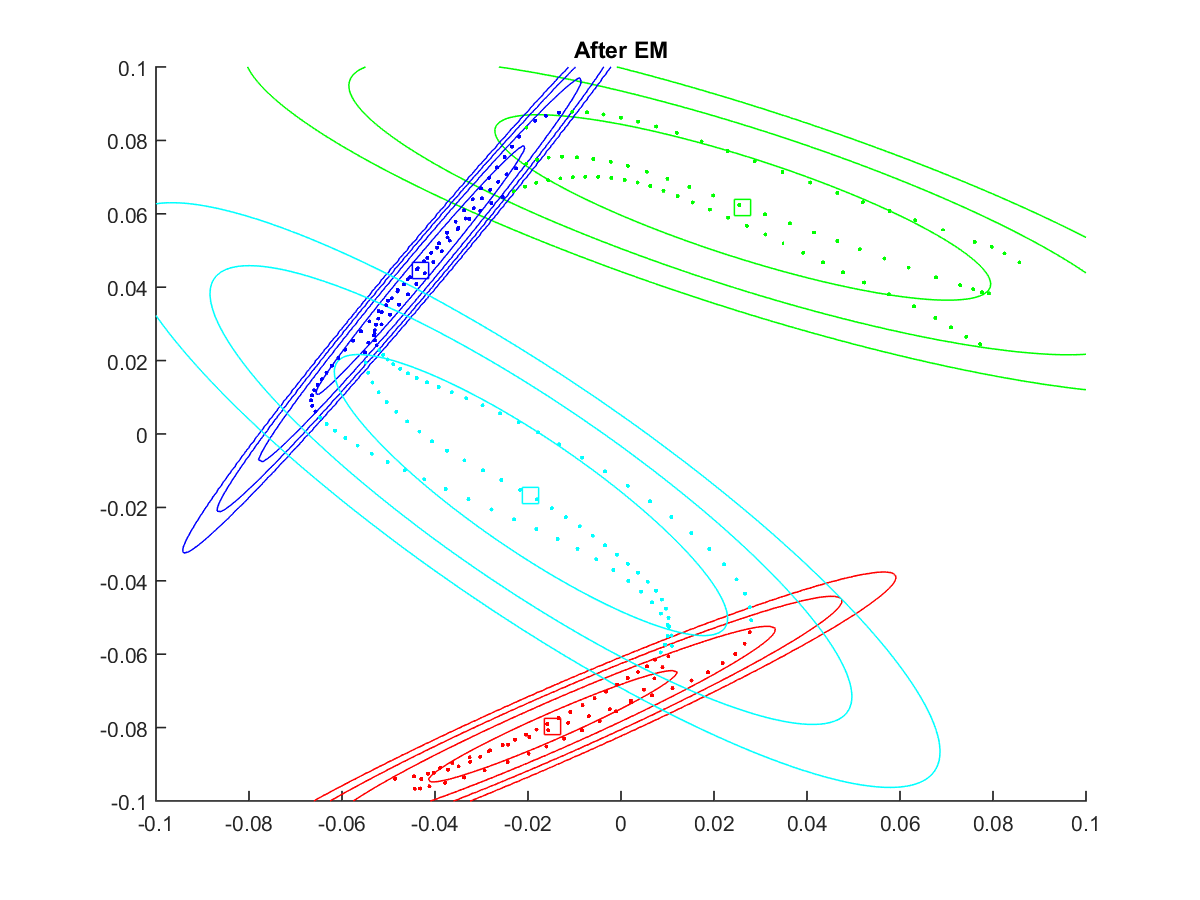
\includegraphics[width=0.5\textwidth]{img/1after_em.png}
    \caption{Gaussians and clusters after EM}
    \label{fig:after_em}
\end{figure}
\newpage
~
\newpage
\section{Exercise}
The following list contains the log-likelihood and the labels of the Train Set. By labeling 1 stands for class \textit{train} and 0 stands for class \textit{test}.
$$
[log-likelihood, label] =
 \begin{smallmatrix}
 %logLH  & class\\
 &-2.312 &1.000\\
 &-2.312 &1.000\\
 &-14.620 &1.000\\
 &-24.359 &1.000\\
 &-46.196 &1.000\\
 &-46.196 &1.000\\
 &-70.710 &1.000\\
 &-87.584 &1.000\\
 &-68.024 &1.000\\
 &-67.401 &1.000\\
 &-89.607 &1.000\\
 &-92.499 &1.000\\
 &-126.337 &0.000\\
 &-115.001 &1.000\\
 &-70.706 &1.000\\
 &-94.465 &1.000\\
 &-115.794 &1.000\\
 &-95.986 &1.000\\
 &-117.905 &1.000\\
 &-81.088 &1.000\\
 &-89.167 &1.000\\
 &-89.331 &1.000\\
 &-50.709 &1.000\\
 &-80.423 &1.000\\
 &-57.664 &1.000\\
 &-40.420 &1.000\\
 &-56.434 &1.000\\
 &-45.929 &1.000\\
 &-45.789 &1.000\\
 &-39.312 &1.000\\
 &-39.312 &1.000\\
 &-39.172 &1.000\\
 &-38.899 &1.000\\
 &-38.348 &1.000\\
 &-38.348 &1.000\\
 &-38.070 &1.000\\
 &-37.936 &1.000\\
 &-37.803 &1.000\\
 &-37.803 &1.000\\
 &-37.669 &1.000\\
 &-37.193 &1.000\\
 &-36.850 &1.000\\
 &-36.583 &1.000\\
 &-36.449 &1.000\\
 &-35.973 &1.000\\
 &-35.630 &1.000\\
 &-35.630 &1.000\\
 &-35.287 &1.000\\
 &-35.287 &1.000\\
 &-34.944 &1.000\\
 &-34.601 &1.000\\
 &-34.258 &1.000\\
 &-34.258 &1.000\\
 &-24.866 &1.000\\
 &-24.866 &1.000\\
 &-24.866 &1.000\\
 &-2.312 &1.000\\
 &-2.312 &1.000\\
 &-2.312 &1.000\\
 &-2.312 &1.000
 \end{smallmatrix}
$$
\newpage
This list contains the log-likelihood of the Test Set. Where again 1 stands for class \textit{train} and 0 stands for class \textit{test}.
$$
[log-likelihood, label] =
 \begin{smallmatrix}
 %logLH  & class\\
 &-24.866 &1.000\\
 &-24.866 &1.000\\
 &-24.866 &1.000\\
 &-24.866 &1.000\\
 &-24.866 &1.000\\
 &-2.312 &1.000\\
 &-2.312 &1.000\\
 &-2.312 &1.000\\
 &-2.312 &1.000\\
 &-25.627 &1.000\\
 &-22.780 &1.000\\
 &-3.707 &1.000\\
 &-3.955 &1.000\\
 &-3.955 &1.000\\
 &-13.694 &1.000\\
 &-13.694 &1.000\\
 &-25.424 &1.000\\
 &-25.424 &1.000\\
 &-25.424 &1.000\\
 &-25.424 &1.000\\
 &-25.424 &1.000\\
 &-25.424 &1.000\\
 &-46.493 &1.000\\
 &-46.493 &1.000\\
 &-25.055 &1.000\\
 &-47.394 &1.000\\
 &-47.109 &1.000\\
 &-81.300 &1.000\\
 &-86.778 &1.000\\
 &-88.363 &1.000\\
 &-67.047 &1.000\\
 &-39.591 &1.000\\
 &-39.591 &1.000\\
 &-39.591 &1.000\\
 &-39.591 &1.000\\
 &-39.591 &1.000\\
 &-39.591 &1.000\\
 &-39.591 &1.000\\
 &-87.250 &1.000\\
 &-97.489 &1.000\\
 &-97.489 &1.000\\
 &-97.489 &1.000\\
 &-112.441 &1.000\\
 &-119.645 &1.000\\
 &-111.566 &1.000\\
 &-95.408 &1.000\\
 &-118.771 &1.000\\
 &-71.210 &1.000\\
 &-71.210 &1.000\\
 &-71.210 &1.000\\
 &-25.774 &1.000\\
 &-25.774 &1.000\\
 &-25.774 &1.000\\
 &-25.774 &1.000\\
 &-25.774 &1.000\\
 &-25.774 &1.000\\
 &-25.774 &1.000\\
 &-25.774 &1.000\\
 &-25.774 &1.000\\
 &-25.774 &1.000
 \end{smallmatrix}
$$
\newpage
\section{Exercise}
\begin{itemize}

\item Policy Iteration

Reward Matrix
$$
R =
 \begin{pmatrix}
 &0.000 &0.000 &0.000 &0.000\\
 &0.000 &1.000 &-10.000 &-5.000\\
 &0.000 &0.000 &-10.000 &-5.000\\
 &0.000 &0.000 &0.000 &0.000\\
 &-10.000 &-5.000 &0.000 &1.000\\
 &0.000 &0.000 &0.000 &0.000\\
 &0.000 &0.000 &0.000 &0.000\\
 &-10.000 &5.000 &0.000 &0.000\\
 &-10.000 &-5.000 &0.000 &0.000\\
 &0.000 &0.000 &0.000 &0.000\\
 &0.000 &0.000 &0.000 &0.000\\
 &-10.000 &5.000 &0.000 &0.000\\
 &0.000 &0.000 &0.000 &0.000\\
 &0.000 &0.000 &-10.000 &5.000\\
 &0.000 &0.000 &-10.000 &5.000\\
 &0.000 &0.000 &0.000 &0.000
 \end{pmatrix}
$$

Used Value of $\gamma$: \\

Iterations required: \\

Results of \textit{WalkPolicyIteration(s)}:

\begin{figure}[h!]
  	\centering
    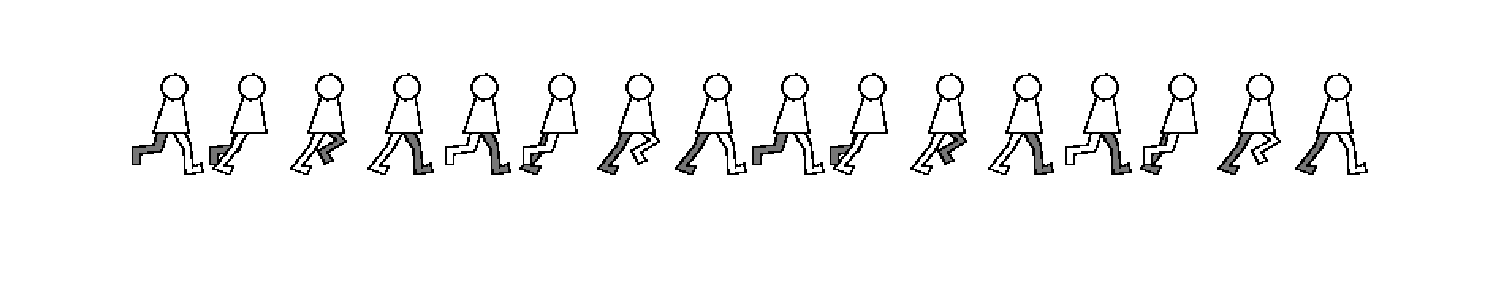
\includegraphics[width=0.5\textwidth]{img/3walkshow8.png}
    \caption{Results from starting state s = 8}
    \label{fig:3walkshow8}
\end{figure}

\begin{figure}[h!]
  	\centering
    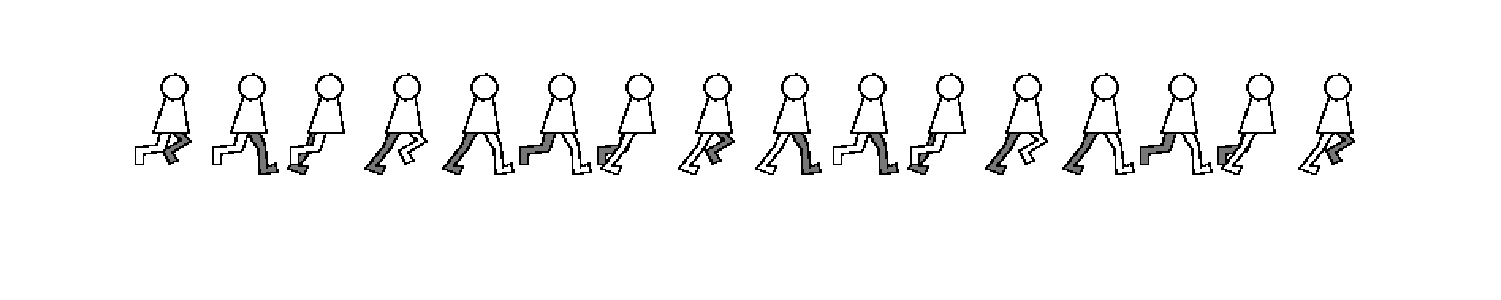
\includegraphics[width=0.5\textwidth]{img/3walkshow10.png}
    \caption{Results from starting state s = 10}
    \label{fig:3walkshow10}
\end{figure}

\begin{figure}[h!]
  	\centering
    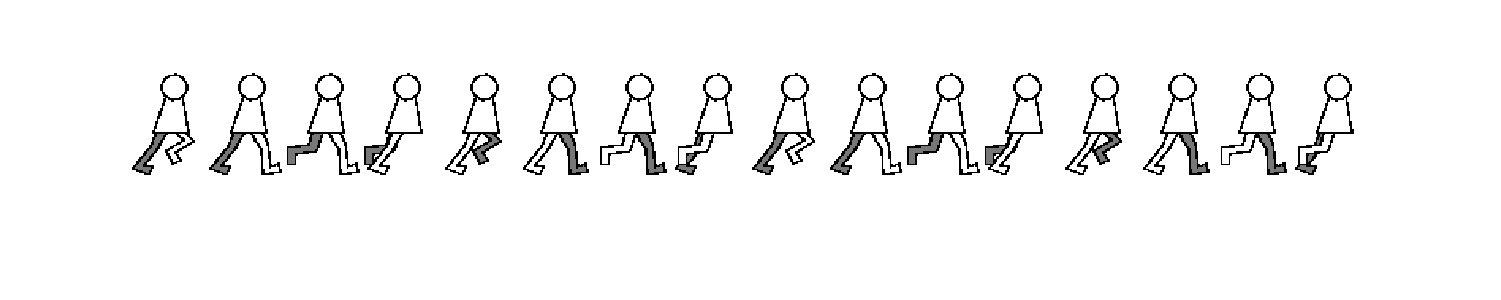
\includegraphics[width=0.5\textwidth]{img/3walkshow3.png}
    \caption{Results from starting state s = 3}
    \label{fig:3walkshow3}
\end{figure}

\item Q-Learning
Used $\epsilon$: \\
Used $\alpha$: \\

Outcomes of changing $\epsilon$ or using pure greedy policy: \\

Steps needed: \\

Results of \textit{WalkQLearning(s)}:
\begin{figure}[h!]
  	\centering
    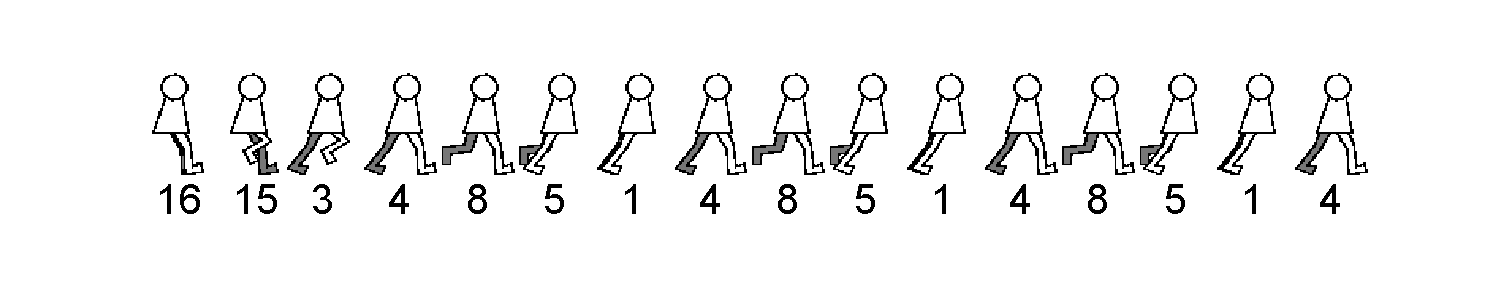
\includegraphics[width=0.5\textwidth]{img/3walkshow16.png}
    \caption{Results from starting state s = 16}
    \label{fig:3walkshow16}
\end{figure}

\begin{figure}[h!]
  	\centering
    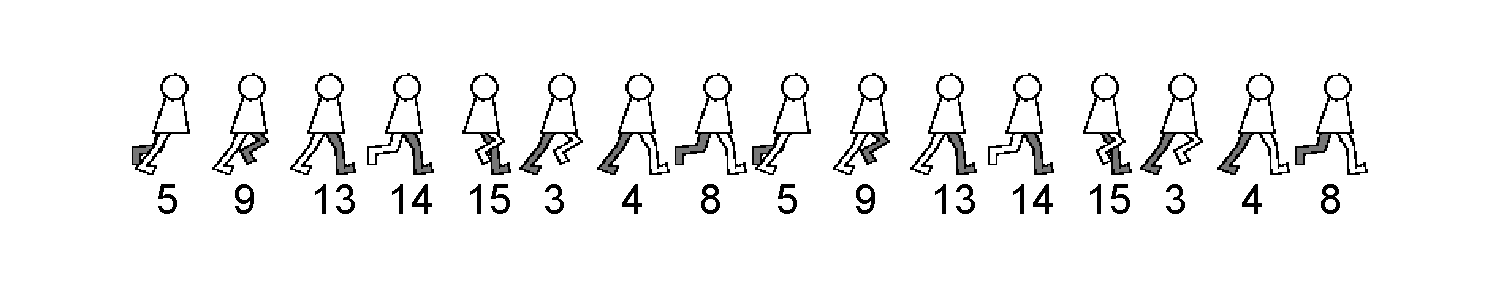
\includegraphics[width=0.5\textwidth]{img/3walkshow5.png}
    \caption{Results from starting state s = 5}
    \label{fig:3walkshow5}
\end{figure}

\begin{figure}[h!]
  	\centering
    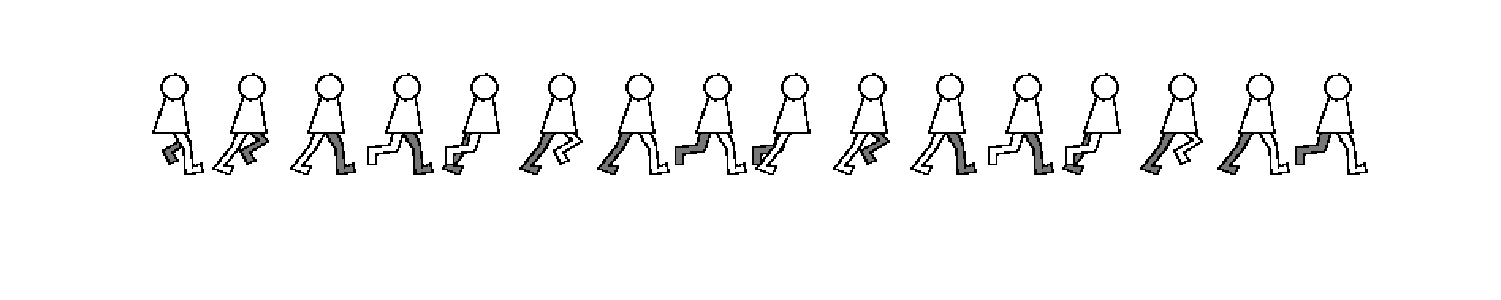
\includegraphics[width=0.5\textwidth]{img/3walkshow12.png}
    \caption{Results from starting state s = 12}
    \label{fig:3walkshow12}
\end{figure}


\end{itemize}
\end{document}


